\chapter{التعرف على المواد}\label{ch:g7:identifying-substances}

يُعثر في مسرح لغز صغير على ورقة مجعّدة كُتبت بقلم لبّاد أسود، ويُعثر في
ثلاث حقائب مختلفة على ثلاثة أقلام لبّاد. تبدو الأحبار الثلاثة للعين بالسواد
نفسه. ولا يحتاج كيميائي الأدلة الجنائية إلا إلى شريط من الورق، وقليل من
الماء، ونصف ساعة ليقول أي قلم كتب الورقة. فالكيميائيون يتعرفون على
المواد لا بمظهرها، بل بسلوكها في اختبار اختير لها.

\begin{recall}
\omterm{def:g6:pure-substances-and-mixtures:species}{النوع الكيميائي} صنف معيّن من المواد؛ \omterm{def:g6:pure-substances-and-mixtures:pure-substance}{والمادة النقية} تحوي نوعًا واحدًا،
\omterm{def:g6:pure-substances-and-mixtures:mixture}{والخليط} عدة أنواع (\cref{ch:g6:pure-substances-and-mixtures}). وبعض
المواد \omterm{def:g2:mixing-and-dissolving:dissolve}{يذوب} جيدًا في \omterm{def:g6:solutions-and-solubility:solute}{مذيب}، وبعضها قليلًا أو لا \omterm{def:g2:mixing-and-dissolving:dissolve}{يذوب} أبدًا: لكل منها
ذوبانيته (\cref{ch:g6:solutions-and-solubility}).
\end{recall}

\section{ما الاختبار المميِّز}

\begin{definition}[الاختبار المميِّز والكاشف]\label{def:g7:identifying-substances:characteristic-test}
\emph{الاختبار المميِّز}\index{اختبار مميز} \omterm{def:g6:pure-substances-and-mixtures:species}{لنوع كيميائي} تجربة بسيطة
تعطي نتيجة مرئية مع هذا النوع، ولا تعطيها مع الأنواع الأخرى التي نلقاها
في الموقف نفسه. ويستعمل مادة مختارة لهذا الغرض هي
\emph{الكاشف}\index{كاشف}.
\end{definition}


\begin{method}[إجراء اختبار مميِّز]\label{met:g7:identifying-substances:run}
\begin{enumerate}
  \item خذ عيّنة صغيرة من المادة المراد اختبارها.
  \item أضف \omterm{def:g7:identifying-substances:characteristic-test}{الكاشف}، أو اجعله يلامس العيّنة، كما يصف
        الاختبار.
  \item لاحظ: تغيّر لون، أو تعكّر، أو لهب، أو صوت.
  \item استنتج: يكون الاختبار \emph{إيجابيًا} إذا ظهرت النتيجة
        المتوقعة، و\emph{سلبيًا} إذا لم تظهر.
  \item أجرِ الاختبار نفسه على عيّنة نعلم أنها لا تحوي النوع
        (وهي الشاهد): يجب أن يبقى سلبيًا، وإلا فالنتيجة لا تثبت
        شيئًا.
\end{enumerate}
\end{method}

\section{أربعة اختبارات تقليدية}

\begin{proposition}[ثنائي أكسيد الكربون يعكّر ماء الجير]\label{prop:g7:identifying-substances:limewater}
ماء الجير \omterm{def:g2:mixing-and-dissolving:dissolve}{محلول} رائق عديم اللون. فإذا مُرّر فيه ثنائي أكسيد الكربون
فقاعاتٍ صار حليبيًا، عكرًا أبيض. \omterm{def:g4:air-a-mixture-of-gases:air}{والهواء} المزفور عبر ماصّة يعكّر ماء
الجير؛ أما \omterm{def:g4:air-a-mixture-of-gases:air}{الهواء} النقي الذي يُضخ فيه فلا يكاد يعكّره.
\end{proposition}

\begin{omfigure}
\begin{tikzpicture}[font=\small, scale=1.25]
  % generating tube, stoppered
  \pic[transform shape] at (0,0) {testtube={0.35}{omWater!80}};
  \fill[black!65] (-0.27,2.8) rectangle (0.27,3.15);
  \foreach \y in {0.4,0.65,0.85} \draw[black!55] (0.05,\y) circle (0.04);
  \pic[transform shape] at (0,2.9) {deliverytube={1.9}{-2.3}};
  % limewater tube
  \pic[transform shape] at (1.9,0) {testtube={0.6}{white!85!black}};
  \foreach \x/\y in {1.88/0.75,1.95/1.0,1.85/1.25,1.92/1.5} \draw[black!55] (\x,\y) circle (0.04);
  \draw[<-, omProp, thick] (-0.3,0.5) -- (-1.2,0.8) node[left, text=black, align=right]
    {تفاعل\\ ينطلق منه غاز};
  \draw[<-, omProp, thick] (2.2,1.2) -- (3.0,1.4) node[right, text=black, align=left]
    {يتعكّر ماء الجير:\\ الغاز هو\\ ثنائي أكسيد الكربون};
\end{tikzpicture}

{\small اختبار ماء الجير. يمر الغاز المنطلق في الأنبوب الأول فقاعاتٍ في
ماء الجير؛ فإذا تعكّر ماء الجير كان الغاز ثنائي أكسيد
الكربون.}
\end{omfigure}

\begin{proposition}[الماء يُزرّق كبريتات النحاس اللامائية]\label{prop:g7:identifying-substances:copper-sulfate}
كبريتات النحاس اللامائية مسحوق أبيض. وقطرة ماء تجعلها زرقاء في الحال.
ويبيّن الاختبار وجود الماء، في سائل أو في جسم صلب رطب --- لا أن السائل
ماء نقي.
\end{proposition}

\begin{omfigure}
\begin{minipage}[b]{0.48\linewidth}\centering
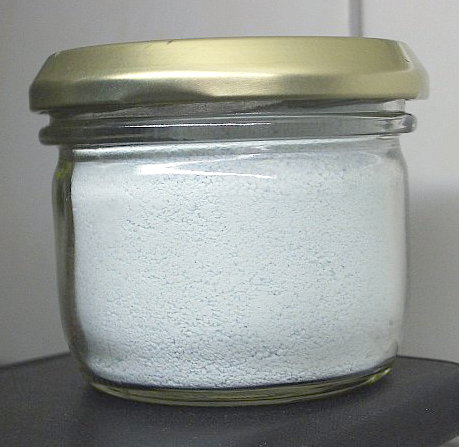
\includegraphics[width=\linewidth,height=4.2cm,keepaspectratio]{images/book1/cuso4-anhydrous.jpg}

{\small كبريتات النحاس اللامائية: مسحوق أبيض. تصوير: ف.~أولن،
CC BY-SA 3.0.}
\end{minipage}\hfill
\begin{minipage}[b]{0.48\linewidth}\centering
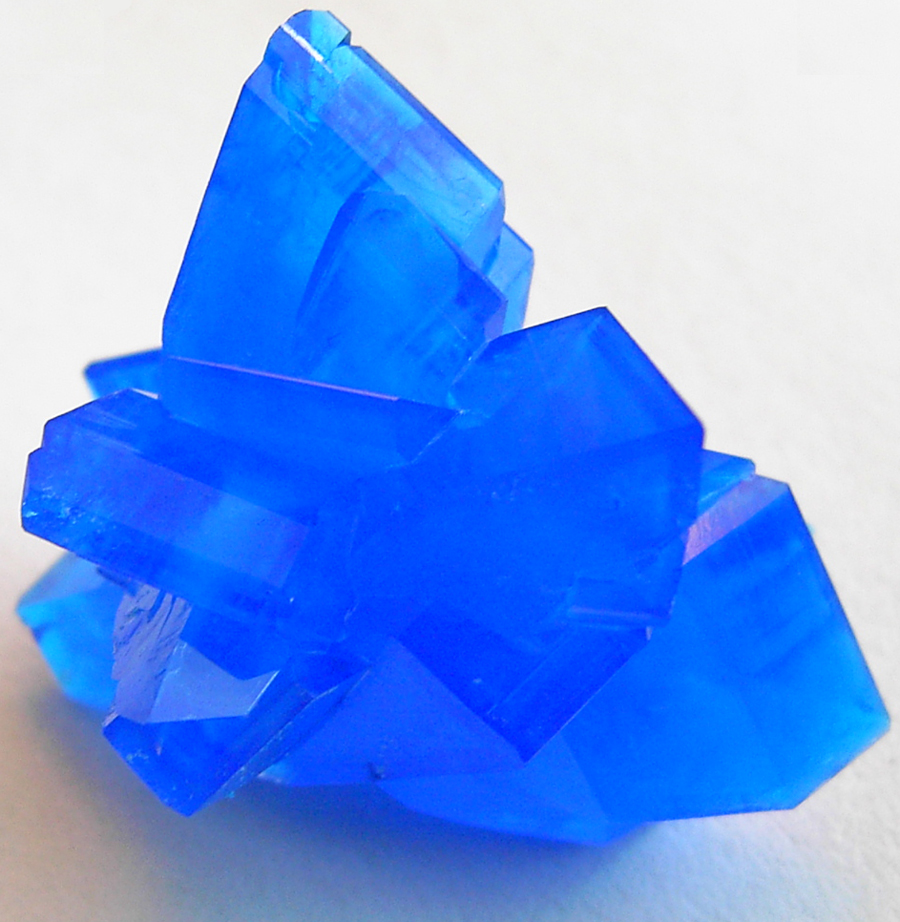
\includegraphics[width=\linewidth,height=4.2cm,keepaspectratio]{images/book1/cuso4-hydrated.jpg}

{\small تصير زرقاء مع الماء؛ وهذه البلورات تحوي ماءً. تصوير:
Stephanb، CC BY-SA 3.0.}
\end{minipage}
\end{omfigure}

\begin{safety}{\ghs[0.82cm]{GHS05}\ghs[0.82cm]{GHS07}\ghs[0.82cm]{GHS09}}
% ledger: ghs:CuSO4
كبريتات النحاس: ضارة إذا ابتُلعت ومهيّجة للجلد (GHS07)؛ وقد تؤذي العينين
أذى بالغًا (GHS05)؛ وشديدة السمية للأحياء المائية، مع آثار طويلة الأمد
(GHS09). نظارات واقية وقفازات؛ وتُجمع النفايات، ولا تُصب أبدًا في
المغسلة.
\end{safety}

\begin{proposition}[الأكسجين يعيد إشعال عود متوهج]\label{prop:g7:identifying-substances:splint}
يُشعل عود خشبي، ثم يُطفأ بالنفخ فلا يبقى منه إلا توهج أحمر. فإذا أُدخل
العود المتوهج في أنبوب اختبار فيه أكسجين عاد يشتعل
لهبًا.
\end{proposition}

\begin{proposition}[الهيدروجين يحترق بفرقعة حادة]\label{prop:g7:identifying-substances:pop}
العود المشتعل الذي يُمسك عند فوهة أنبوب اختبار صغير فيه هيدروجين يُحدث
«فرقعة» قصيرة حادة: فالهيدروجين يحترق فورًا مع أكسجين
\omterm{def:g4:air-a-mixture-of-gases:air}{الهواء}.
\end{proposition}

\begin{omfigure}
\begin{tikzpicture}[font=\small, scale=1.25]
  % splint test for oxygen
  \pic[transform shape] at (0,0) {testtube={0}{white}};
  \draw[brown!60!black, line width=2pt] (0.15,1.6) -- (1.4,3.6);
  \fill[orange!85] (0.15,1.6) circle (0.07);
  \fill[orange!80] (0.12,1.62) .. controls (0.0,1.9) and (0.08,2.1) .. (0.1,2.3)
    .. controls (0.2,2.05) and (0.3,1.85) .. (0.2,1.62);
  \node[anchor=north, align=center] at (0,-0.15) {الأكسجين:\\ العود المتوهج\\ يشتعل لهبًا};
  % pop test for hydrogen
  \begin{scope}[xshift=4cm]
    \pic[transform shape, rotate=180] at (0,3.1) {testtube={0}{white}};
    \draw[brown!60!black, line width=2pt] (0.05,-0.05) -- (1.3,-0.9);
    \fill[orange!85] (0.05,-0.02) .. controls (-0.05,0.08) and (0.0,0.15) .. (0.02,0.22)
      .. controls (0.08,0.15) and (0.15,0.08) .. (0.1,-0.02);
    \node[font=\small\itshape] at (-0.9,0.15) {فرقعة!};
    \node[anchor=north, align=center] at (0,-1.0) {الهيدروجين:\\ فرقعة حادة\\ عند الفوهة};
  \end{scope}
\end{tikzpicture}

{\small يسارًا: عود متوهج يعود فيشتعل في الأكسجين. يمينًا: عود مشتعل عند
فوهة أنبوب مقلوب فيه هيدروجين يُحدث فرقعة حادة (الهيدروجين أخف من \omterm{def:g4:air-a-mixture-of-gases:air}{الهواء}،
ولذلك يُمسك الأنبوب وفوهته إلى الأسفل).}
\end{omfigure}

\begin{safety}{\ghs[0.82cm]{GHS02}\ghs[0.82cm]{GHS04}}
% ledger: ghs:H2
الهيدروجين: غاز شديد القابلية للاشتعال (GHS02)، يُخزَّن تحت الضغط في
أسطوانات (GHS04). ولا يُجرى اختبار الفرقعة إلا ببضعة ميليلترات، ويُجريه
المعلم.
\end{safety}

\section{الكروماتوغرافيا الورقية}

\begin{definition}[الكروماتوغرافيا الورقية والكروماتوغرام]\label{def:g7:identifying-substances:chromatography}
\emph{الكروماتوغرافيا الورقية}\index{كروماتوغرافيا ورقية} تفصل صبغات
\omterm{def:g6:pure-substances-and-mixtures:mixture}{خليط}. توضع بقعة صغيرة من \omterm{def:g6:pure-substances-and-mixtures:mixture}{الخليط} على خط مرسوم قرب أسفل شريط من الورق؛
ويُغمس أسفل الشريط في \omterm{def:g6:solutions-and-solubility:solute}{مذيب} يصعد ببطء في الورق ويحمل معه كل صبغة، بعضها
أسرع من بعض. وحين يكاد \omterm{def:g6:solutions-and-solubility:solute}{المذيب} يبلغ أعلى الشريط يُخرج الشريط ويُجفف: فهو
\emph{الكروماتوغرام}\index{كروماتوغرام}.
\end{definition}

\begin{omfigure}
\begin{tikzpicture}[font=\small, scale=1.3]
  % the strip in a beaker of solvent
  \pic[transform shape] at (0,0) {beaker={0.12}{omWater!80}};
  \fill[white] (-0.42,0.06) rectangle (0.42,2.2);
  \fill[omWater!80] (-0.42,0.06) rectangle (0.42,0.24);
  \draw[omGlass, line width=0.6pt] (-0.42,0.06) rectangle (0.42,2.2);
  \draw[black!60, line width=0.4pt] (-0.42,0.42) -- (0.42,0.42);
  \fill[black!80] (0,0.42) circle (0.07);
  \shade[ball color=black!20] (0,2.27) circle (0.08);
  \draw[black!50, line width=1.2pt] (-1.1,2.27) -- (1.1,2.27);
  \node[anchor=north, align=center] at (0,-0.15) {في البداية};
  \draw[<-, omProp, thick] (0.1,0.5) -- (1.3,0.8) node[right, text=black]
    {بقعة حبر على خط بقلم الرصاص};
  \draw[<-, omProp, thick] (1.0,2.27) -- (1.3,2.5) node[right, text=black]
    {ساق زجاجية تمسك الورقة};
  \draw[<-, omProp, thick] (0.75,0.15) -- (1.3,0.25) node[right, text=black]
    {المذيب، تحت الخط};
  % the chromatogram
  \begin{scope}[xshift=6.2cm]
    \pic[transform shape] at (0,0) {tlcplate};
    \draw[black!50, dashed] (-0.7,2.7) -- (0.7,2.7);
    \fill[blue!70] (0,1.0) ellipse (0.13 and 0.09);
    \fill[red!70] (0,1.7) ellipse (0.13 and 0.09);
    \fill[yellow!80!orange] (0,2.35) ellipse (0.13 and 0.09);
    \node[anchor=north, align=center] at (0,-0.15) {الكروماتوغرام};
    \draw[<-, omProp, thick] (0.75,2.7) -- (1.3,2.85) node[right, text=black]
      {المسافة التي صعدها المذيب};
    \draw[<-, omProp, thick] (0.2,1.7) -- (1.3,1.7) node[right, text=black]
      {ثلاث صبغات: الحبر خليط};
  \end{scope}
\end{tikzpicture}

{\small \omterm{def:g7:identifying-substances:chromatography}{الكروماتوغرافيا الورقية} لحبر أسود. يصعد \omterm{def:g6:solutions-and-solubility:solute}{المذيب} في الورق ويفصل
الحبر إلى ثلاث صبغات.}
\end{omfigure}

\begin{method}[قراءة الكروماتوغرام]\label{met:g7:identifying-substances:read}
\begin{enumerate}
  \item عُدّ البقع فوق كل نقطة انطلاق: بقعة واحدة تعني صبغة واحدة؛
        وبقعتان أو أكثر تعني خليطًا من الصبغات.
  \item قارن الارتفاعات: في \omterm{def:g7:identifying-substances:chromatography}{الكروماتوغرام} الواحد تصعد الصبغة الواحدة
        دائمًا إلى الارتفاع نفسه. والبقعة التي في ارتفاع صبغة معروفة
        هي على الأرجح تلك الصبغة.
  \item ارسم الخط بقلم الرصاص، لا بالحبر أبدًا: فالحبر نفسه سيفصله
        \omterm{def:g6:solutions-and-solubility:solute}{المذيب}.
\end{enumerate}
\end{method}

\begin{example}[صبغات الحلوى]\label{ex:g7:identifying-substances:sweets}
تُكشط الأغلفة الملونة لحبات الحلوى في قليل من الماء، وتوضع بقعًا على شريط
إلى جانب بقع من صبغات الطعام المسموح بها في الحلوى. فيبيّن \omterm{def:g7:identifying-substances:chromatography}{الكروماتوغرام} أن
الغلاف الأخضر يحوي صبغة صفراء وصبغة زرقاء، وكلتاهما من الصبغات
المسموح بها.
\end{example}


\section{قراءة جدول الاختبارات}

\begin{proposition}[جدول الاختبارات المميِّزة]\label{prop:g7:identifying-substances:bank}
يحفظ الكيميائيون الاختبارات التي يستعملونها في جدول، هو جدول الاختبارات،
ويُقرأ من اليمين إلى اليسار:
\begin{center}
\small
\begin{tabular}{llll}
\hline
النوع المبحوث عنه & \omterm{def:g7:identifying-substances:characteristic-test}{الكاشف} أو الاختبار & النتيجة الإيجابية & \\
\hline
ثنائي أكسيد الكربون & ماء الجير & يتعكّر ماء الجير & \\
الماء & كبريتات النحاس اللامائية & يصير الأبيض أزرق & \\
الأكسجين & عود متوهج & يعود العود فيشتعل & \\
الهيدروجين & عود مشتعل & فرقعة حادة & \\
صبغات \omterm{def:g6:pure-substances-and-mixtures:mixture}{خليط} & \omterm{def:g7:identifying-substances:chromatography}{الكروماتوغرافيا الورقية} & بقعة لكل صبغة & \\
\hline
\end{tabular}
\end{center}
\end{proposition}

\begin{remark}[ما لا يقوله الاختبار]\label{rem:g7:identifying-substances:limits}
الاختبار الإيجابي يثبت أن النوع موجود، لا أنه وحده: فالسائل الذي يُزرّق
كبريتات النحاس يحوي ماءً، لكنه قد يكون ماءً مالحًا أو عصير برتقال. أما
الاختبار السلبي فلا يقول إلا إن النوع غائب، أو موجود بمقدار أصغر من أن
يظهر.
\end{remark}

\begin{omfigure}
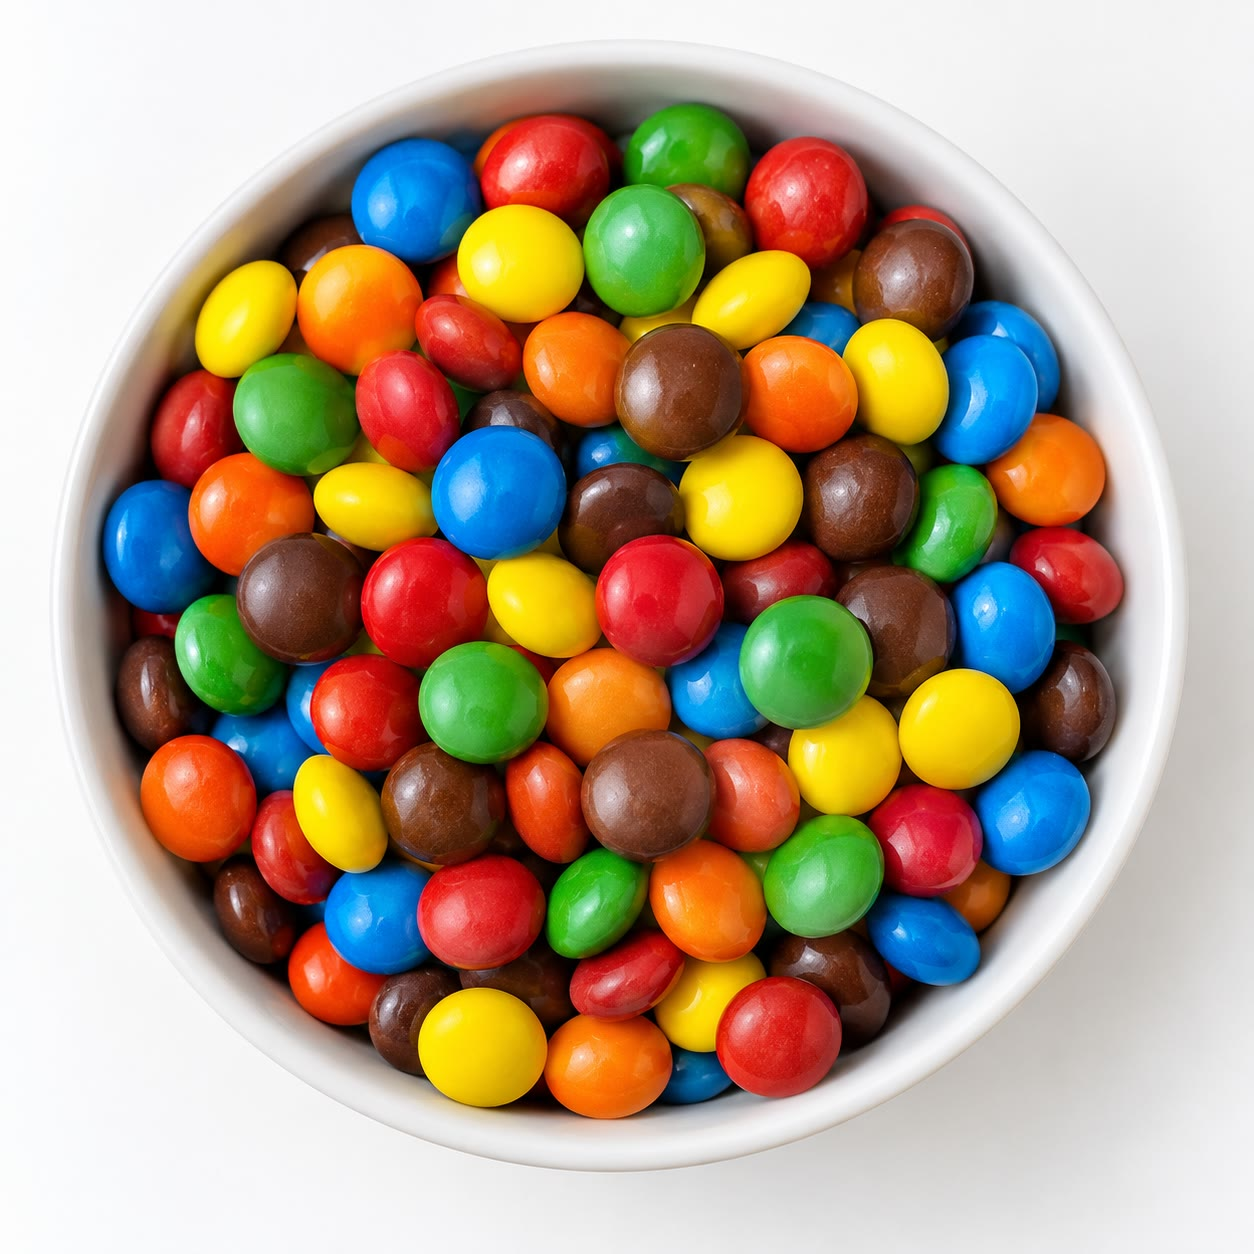
\includegraphics[width=0.32\linewidth]{images/book1/ai/g7-sweets.jpg}

{\small حبات حلوى ملبّسة بالسكر: ألوانها خلائط من صبغات يمكن للكروماتوغرافيا
أن تفصلها.}
\end{omfigure}

\begin{omfigure}
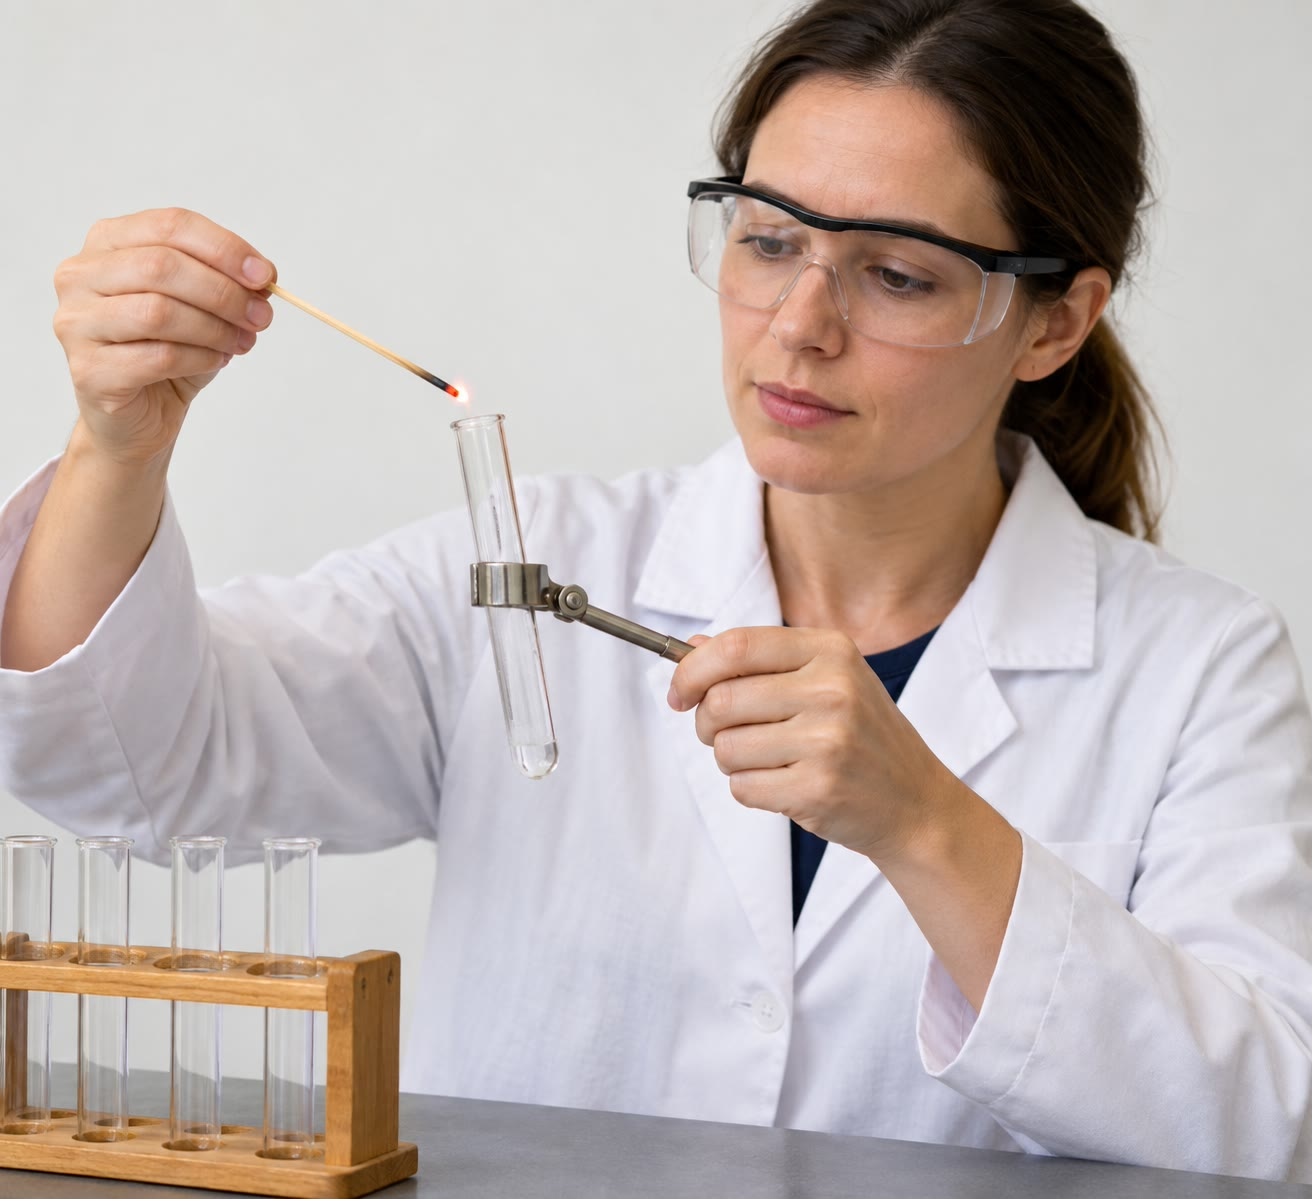
\includegraphics[width=0.36\linewidth]{images/book1/ai/g7-splint-teacher.jpg}

{\small معلمة تختبر غازًا بعود متوهج.}
\end{omfigure}

\section{تمارين}

\begin{exercise}[$\star$]\label{exo:g7:identifying-substances:1}
أي اختبار يتعرف على ثنائي أكسيد الكربون؟ صف نتيجته الإيجابية.
\end{exercise}

\begin{exercise}[$\star$]\label{exo:g7:identifying-substances:2}
مسحوق أبيض يصير أزرق حين يُقطر عليه سائل. ماذا يبيّن هذا عن
السائل؟
\end{exercise}

\begin{exercise}[$\star$]\label{exo:g7:identifying-substances:3}
يوضع عود متوهج في مخبار غاز فيعود يشتعل لهبًا. أي غاز في
المخبار؟
\end{exercise}

\begin{exercise}[$\star$]\label{exo:g7:identifying-substances:4}
لماذا يُرسم خط الانطلاق في \omterm{def:g7:identifying-substances:chromatography}{الكروماتوغرافيا الورقية} بقلم الرصاص لا
بالحبر؟
\end{exercise}

\begin{exercise}[$\star\star$]\label{exo:g7:identifying-substances:5}
لماذا يجب أن يكون خط الانطلاق فوق مستوى \omterm{def:g6:solutions-and-solubility:solute}{المذيب} في
الكأس؟
\end{exercise}

\begin{exercise}[$\star\star$]\label{exo:g7:identifying-substances:6}
يبيّن \omterm{def:g7:identifying-substances:chromatography}{كروماتوغرام} حبر أخضر بقعتين، إحداهما في ارتفاع صبغة مرجعية صفراء،
والأخرى في ارتفاع صبغة مرجعية زرقاء. هل الحبر الأخضر \omterm{def:g6:pure-substances-and-mixtures:pure-substance}{مادة نقية}؟ ومِمَّ
يتكون؟
\end{exercise}

\begin{exercise}[$\star\star$]\label{exo:g7:identifying-substances:7}
مستعينًا بجدول الاختبارات، أي اختبار تستعمل لتبيّن أن غازًا منطلقًا من تفاعل
هو الهيدروجين؟ وماذا تتوقع أن ترى؟
\end{exercise}

\begin{exercise}[$\star\star$]\label{exo:g7:identifying-substances:8}
\omterm{def:g4:air-a-mixture-of-gases:air}{الهواء} المزفور يعكّر ماء الجير أسرع بكثير من \omterm{def:g4:air-a-mixture-of-gases:air}{الهواء} النقي. ماذا يخبرنا
هذا عن \omterm{def:g4:air-a-mixture-of-gases:air}{الهواء} الذي نزفره؟
\end{exercise}

\begin{exercise}[$\star\star$]\label{exo:g7:identifying-substances:9}
سائل رائق يُزرّق كبريتات النحاس اللامائية. فيستنتج سام: «إنه ماء
نقي.» اشرح لماذا أخطأ سام.
\end{exercise}

\begin{exercise}[$\star\star$]\label{exo:g7:identifying-substances:10}
انظر إلى \omterm{def:g7:identifying-substances:chromatography}{كروماتوغرام} الحبر الأسود في هذا الفصل. كم صبغة يحوي الحبر؟
وأي صبغة صعدت أعلى من غيرها؟
\end{exercise}

\begin{exercise}[$\star\star\star$]\label{exo:g7:identifying-substances:11}
ثلاثة مخابير فيها الأكسجين والهيدروجين وثنائي أكسيد الكربون، لكن ملصقاتها
ضاعت. خطّط على الورق للاختبارات التي تسمّي كل مخبار، بترتيب يستعمل أقل
عدد ممكن من الاختبارات.
\end{exercise}

\begin{exercise}[$\star\star\star$]\label{exo:g7:identifying-substances:12}
يختبر تلميذ غازًا بماء الجير فلا يرى شيئًا يحدث. أعطِ تفسيرين ممكنين،
واختبار الشاهد الذي يساعد على الحسم.
\end{exercise}

\section{مسألة: الورقة المزوّرة}

\begin{problem}[{مسألة نهاية الأسبوع --- ورقة بقلم لبّاد، وثلاثة أقلام
مشبوهة، وثلاث أسطوانات غاز بلا ملصقات، وجدول اختبارات}]
\label{pb:g7:identifying-substances:1}
يُطلب من مختبر مدرسي أن يساعد في حل لغزين صغيرين. الأول: يجب ربط ورقة
كُتبت بقلم لبّاد أسود بواحد من ثلاثة أقلام سوداء، 1 و2 و3. تؤخذ قطرة
حبر من الورقة ومن كل قلم، وتوضع بقعًا على شريط الورق نفسه، ثم يُنشر الشريط
بالماء. \omterm{def:g7:identifying-substances:chromatography}{والكروماتوغرام} مبيّن أدناه.
\begin{center}
\begin{tikzpicture}[font=\small, x=1cm, y=1cm]
  \fill[white] (0,0) rectangle (6,4);
  \draw[omGlass, line width=0.6pt] (0,0) rectangle (6,4);
  \draw[black!60] (0,0.5) -- (6,0.5);
  \draw[black!50, dashed] (0,3.6) -- (6,3.6);
  \foreach \x/\lab in {0.9/الورقة, 2.3/القلم 1, 3.7/القلم 2, 5.1/القلم 3}
    \node[anchor=north] at (\x,-0.05) {\lab};
  % note: three dyes
  \fill[blue!70] (0.9,1.2) ellipse (0.18 and 0.1);
  \fill[red!70] (0.9,2.2) ellipse (0.18 and 0.1);
  \fill[yellow!80!orange] (0.9,3.1) ellipse (0.18 and 0.1);
  % pen 1: two dyes
  \fill[blue!70] (2.3,1.2) ellipse (0.18 and 0.1);
  \fill[black!70] (2.3,2.7) ellipse (0.18 and 0.1);
  % pen 2: same three as the note
  \fill[blue!70] (3.7,1.2) ellipse (0.18 and 0.1);
  \fill[red!70] (3.7,2.2) ellipse (0.18 and 0.1);
  \fill[yellow!80!orange] (3.7,3.1) ellipse (0.18 and 0.1);
  % pen 3: three dyes, other heights
  \fill[violet!70] (5.1,0.9) ellipse (0.18 and 0.1);
  \fill[red!70] (5.1,1.8) ellipse (0.18 and 0.1);
  \fill[green!60!black] (5.1,2.6) ellipse (0.18 and 0.1);
  \node[anchor=west, font=\footnotesize] at (6.1,3.6) {جبهة المذيب};
  \node[anchor=west, font=\footnotesize] at (6.1,0.5) {خط الانطلاق};
\end{tikzpicture}
\end{center}

\medskip
\noindent\textbf{الجزء الأول --- \omterm{def:g7:identifying-substances:chromatography}{الكروماتوغرام}.}
\begin{enumerate}
  \item لماذا وُضعت الأحبار الأربعة كلها على الشريط نفسه ونُشرت
        معًا؟
  \item هل حبر الورقة \omterm{def:g6:pure-substances-and-mixtures:pure-substance}{مادة نقية} أم \omterm{def:g6:pure-substances-and-mixtures:mixture}{خليط}؟ علّل.
  \item كم صبغة يحوي حبر القلم 1؟ وهل يمكن أن يكون القلم 1 قد
        كتب الورقة؟
  \item القلم 3 يحوي أيضًا ثلاث صبغات. لماذا لا يمكن أن يكون قد كتب
        الورقة؟
  \item أي قلم يطابق الورقة؟ علّل مستعينًا بارتفاعات
        البقع.
\end{enumerate}

\medskip
\noindent\textbf{الجزء الثاني --- ثلاث أسطوانات غاز.}
اللغز الثاني: ثلاث أسطوانات صغيرة، X وY وZ، ضاعت ملصقاتها؛ وهي تحوي
الأكسجين والهيدروجين وثنائي أكسيد الكربون. يُجمع قليل من غاز كل منها في
أنبوب اختبار. الغاز X يعيد إشعال عود متوهج. والغاز Y يُحدث فرقعة حادة
مع عود مشتعل. والغاز Z يعكّر ماء الجير.
\begin{enumerate}[resume]
  \item سمِّ الغاز X.
  \item سمِّ الغاز Y.
  \item سمِّ الغاز Z.
  \item قبل اختبار الغاز Z يمرّر التلميذ هواءً عاديًا في ماء الجير نفسه
        المدة نفسها، فيبقى رائقًا. ماذا يسمى هذا الاختبار الثاني، وماذا
        يضيف إلى الاستنتاج؟
\end{enumerate}

\medskip
\noindent\textbf{الجزء الثالث --- جدول الاختبارات.}
\begin{enumerate}[resume]
  \item سائل عديم اللون وُجد بجانب الورقة يُزرّق كبريتات النحاس
        اللامائية. اكتب سطر جدول الاختبارات المستعمل، وما تبيّنه
        النتيجة.
  \item هل تثبت هذه النتيجة أن السائل ماء نقي؟ علّل.
  \item اختم اللغز الأول: كم صبغة يحوي حبر الورقة، وأي قلم
        كتبها؟
\end{enumerate}
\end{problem}
